% ======== Template para elaboracion de informes ========
% version: 1.3  - Jul/12 
% autor: www.fing.edu.uy/~jperez 
% =======================================================
%
% ----- LICENCIA -----
% Este trabajo es distribuido bajo la licencia LaTeX Project Public License
% Puede y DEBE ser usado, modificado y distribuido gratuitamente.
%
% This work is distributed under the LaTeX Project Public License (LPPL)
% ( http://www.latex-project.org/ ). Must and may be freely used,
% distributed and modified.
% ---------------------
%
%
% ----- INSTRUCCIONES -----
% ver readme
% compilacion:  PdfLaTeX
%
% **************************************************************************

%\documentclass[a4paper,11pt]{article} 
%\documentclass[a4paper,11pt]{report} 
\documentclass[a4paper,11pt]{report}


% ===== Algunos paquetes a ser usados =====

% para poder escribir con tildes
\usepackage[T1]{fontenc}
%\usepackage[utf8]{inputenc}
\usepackage[spanish]{babel}
%\usepackage[utf8]{inputenc}

% fuentes para escribir símbolos
\usepackage{amsfonts}
\usepackage{amssymb}
\usepackage{amsthm}
\usepackage{mathrsfs}

% inclusión de graficos
\usepackage{graphicx}

\usepackage{hyperref}
\pagestyle{empty}
\usepackage[centertags]{amsmath}
\usepackage[utf8x]{inputenc} 

\newcommand{\degree}{\ensuremath{^\circ}}

% ====================================
\usepackage{apacite}
\usepackage{verbatim} 

%\usepackage{cite}
%sudo apt-get install texlive-bibtex-extra
	



% ===== Encabezado =====
\pagestyle{myheadings}
%\markright{Informe número 01 \hfill Tecnología y Sociedad \hfill}
%\markright{Modelo para la detección de avalanchas en secuencias de video:Caso Laguna Palcacocha}
% ======================


% ===== Ajuste layout pagina =====
%\usepackage{fullpage}
\oddsidemargin=-.25cm
\setlength{\textwidth}{160mm}
\setlength{\textheight}{210mm}
\addtolength{\voffset}{-5pt}
% ================================

% --- commandos ---
\newcommand{\ds}{\displaystyle}
\def\x{{\bf x}}
% -----------------



% ========  Aca comienza el cuerpo del texto ==========


\title{Modelo para la detección de avalanchas en secuencias de vídeo :Caso Laguna Palcacocha }
\author{Milwart R. Calizaya Bobadilla}
%\date{\small{24 de Julio del 2019}}

\begin{document}

% hace título
\maketitle

%\newpage

 \chapter{Introducción}
%\section{Introducción }
Las avalanchas, tsunamis, terremotos son los fenómenos naturales  mas destructivos  y ocurren en Perú y el mundo y han causado daños materiales y vidas humanas. 
si bien existen sensores como  LiDAR (Light Detection And Ranging), y Radar (Radio Detection And Ranging), que se utilizaron en estudio de nieve, detección de avalanchas,etc. existen otros sensores acústicos, infrasonido y de fibra óptica 
que si bien no estudian directamente avalanchas se pueden aplicar a otro tipo de movimientos de masa entre ellos avalanchas, por otro lado se ha masificado el uso de  cámaras para video vigilancia, en investigación el uso de videos se ha visto limitado a entornos controlados, ya que en entornos reales se tiene problemas como  la iluminación, resolución, movimiento, etc. la presente investigación se centra en el desarrollo de un modelo para la detección de avalanchas en secuencias de video en la laguna Palcacocha.





\begin{comment}
Se prevee que las avalanchas iran en aumento producto del cambio climático es por eso que hoy resulta importante estudiar su comportamiento, existen muchas técnicas y sensores que pueden ser usados en detección de avalanchas,  y estos pueden ser activos	 o pasivos de acuerdo  a como interactúan con el objeto de estudio, los sensores activos como LiDAR (Light Detection And Ranging), y Radar (Radio Detection And Ranging), y usan partes especificas del espectro electromagnético, miden la radiación emitida por la superficie \cite{Eckerstorfer2016}, algunas investigaciones usan LiDAR \cite{Deems2013} y  otras  Radar \cite{Schimmel2017,Long2016};a pesar de que estos sensores son buenos para la noche, son muy costosos y los pasivos usan el reflejo de la luz solar del espectro electromagnético visible o infra rojo cercano \cite{Fuchs2019}, y sensores de sonido con los avances tecnológicos y la reducción de costos, el uso de estos, especialmente cámaras se ha extendido y se usan cada ves con mas frecuencia en el área de visión computacional  \cite{Jesus2018},y uno de los primeros trabajos en los que en los que se usa fotografiá para estudiar el comportamiento de la nieve\cite{Christiansen2001}; existen otros trabajos para monitorerar  deslizamientos de avalanchas con fotografiás estos trabajos tratan de monitorizar el desplazamiento mediante el conteo de pixeles negros en fotografiás continuas generalmente tomadas en un intervalo de 15 minutos \cite{Thesis2014,Herwijnen2012,Herwijnen2013}; también \cite{Herwijnen2012}, Primero: recomienda que el angulo de visión de la cámara y la pendiente deben de estar lo mas cerca posible a  90 grados; Segundo:La cámara deberá de tener buen acercamiento en el área de interés para para obtener mejores datos; Tercero:el intervalo entre imágenes deberían de tener como máximo ya que las avalanchas surgen rápidamente después de las grietas; por lo tanto  se entiende que un monitoreo en tiempo real seria lo ideal no solamente para monitorizar grietas; si no también avalanchas en ese sentido el uso de videos para estudiar eventos anómalos se ha masificado, existen investigaciones que hacen uso de video para el estudio de avalanchas \cite{Akitaya1980,Nishimura1993}; 




sobre todo en  monitoreo y predicción de movimiento de masa y deslizamiento de tierra que también pueden ser aplicables a avalanchas.


lo sensores remotos pueden ser pasivos o activos, los pasivos pueden usar el reflejo de la luz solar en el espectro electromagnético visible  o infra rojo cercano. 
Se tiene el uso de sensores remotos y estos pueden ser pasivos o activos  como LIDAR y RADAR  que son sensores laser y tambien se otros trabajos se usa sensores acusticos y de infrasonido y de fibra optica, en cuanto a imagenes se tienen trabajos de covertura de nieve \cite{Christiansen2001}, \cite{Bessason2007} donde se pone en evidencia las complicaciones de usar estos este tipo de técnicas durante la noche, y en cuanto a videos no se encontraron trabajos relacionados pero




algunas de las desventajas  serian lo inaccesible del terreno o lo peligroso de su implantacion, es por eso que se hace uso de radares
como los lidar y sar para la deteccion de movientos de masa y deslizamientos de tierra.



\end{comment}




\begin{comment}
En años anteriores se han producido catástrofes en el mundo, tsunamis, terremotos, incendios, inundaciones que  han causado  muchos daños en  materiales y  vidas humanas, y es por eso que se está investigando cómo prevenir, monitorear ciertos eventos como por ejemplo la detección temprana de incendios, o la detección de humo, o la detección de rostros o detección de acciones violentas en secuencias de vídeo, y con lo que respecta a pronóstico de avalanchas se utilizan métodos de control pasivo y activo que muchas veces es muy costoso, es por eso que quiere realizar investigación en   detección de avalancha en secuencias de video que a la fecha no existen a pesar de que se ha masificado el uso de cámaras en otras investigaciones.
La presente investigación se centra en proponer un nuevo modelo para la detección de avalanchas en secuencias de video. Los resultados esperados son: El modelo es eficiente en detección  de Avalanchas en secuencias de video.
\end{comment}





\section{Justificación}
El Perú tiene un largo historial de eventos desastrosos sobre todo en la cordillera blanca, los eventos más recordados y  catastróficos en  Perú ocurrieron en 1962, 1970 donde se desprendió el pico norte del nevado Huascarán provocando una avalancha en Yungay y alrededor de 6000 a 7000 muertes \cite{Evans2009} y otro evento de gran magnitud fue el evento ocurrido en Huaraz el 13 de diciembre de 1941, donde fallecieron 1800 personas \cite{WegnerSteven2014} a causa del desprendimiento de un enorme glaciar en la laguna Palcacocha;en ambos casos los eventos sucedieron a causa de avalanchas, es por eso que la detección de avalanchas es crucial para personas y poblaciones. más aún por los efectos del cambio climático que derriten masas de hielo en los polos y la cordillera, lo que produce mayor riesgo de avalanchas.
La presente investigación pretende con el modelo desarrollado ayudar   mitigar el riesgo frente a una inminente avalancha.

\subsection{Lugar de Estudio:Laguna Palcacocha}

El presente trabajo trata de resolver el problema de la detección de avalanchas en la laguna Palcacocha que se encuentra ubicada en la ciudad de Huaraz(Figura 1), capital del departamento de Ancash, que tiene una población de 140 mil habitantes  que históricamente sufrió eventos extremos como el aluvión del 13 de diciembre de 1941, , a causa de un desprendimiento de un enorme glaciar en la laguna Palcacocha que esta localizada en 9°23’S, 77°22’W, sobre los 4562 m.s.m.m., perteneciente al distrito de Independencia, Provincia de Huaraz, departamento de Ancash \cite{Somos-Valenzuela2016}. Tiene un volumen de alrededor de 17.4 millones de m3 y aunque existe un gran interés en los trabajos de prevención ante un potencial aluvión debido al desborde de la laguna Palcacocha.



\begin{comment}
además de eso en el último inventario de glaciares (INAIGEM 2018a) se ha estimado que el resultado potencial de un aluvión generado en Palcacocha podría ocasionar alrededor de 50 mil víctimas mortales y pérdidas económicas estimada por aluvión: 9 mil millones de soles.
\end{comment}


\begin{figure}[h]
	\centering
	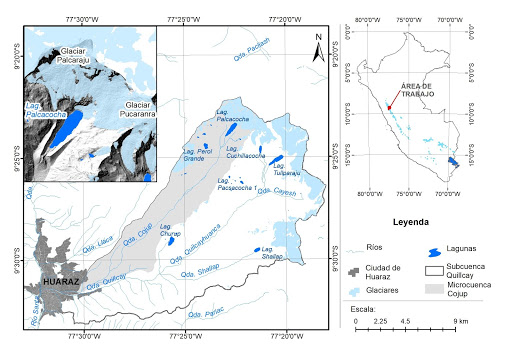
\includegraphics[scale=0.8]{palcacocha}
	\caption{Palcacocha}
	\label{fig:Ubicacion de la laguna Palcacocha}
\end{figure}

\section{Relevancia}
 
 Teniendo en cuenta  que los sensores activos como LiDAR (Light Detection And Ranging), y Radar (Radio Detection And Ranging), etc. se usan para la detección de avalanchas, movimientos de masa, etc. y son precisos pero costosos y los sensores pasivos en muchos casos son menos costosos pero se ven limitados por lo peligroso de su implantación, mantenimiento o  como en el caso de video que a pesar de que se tiene la información en tiempo real se ven limitados por la iluminación, resolución  y condiciones del climáticas, y la presente investigación pretende presentar un modelo para la detección de avalanchas en video no muy costo pero eficiente. En cuanto a otras investigaciones no se encontraron trabajos relacionados a detección de avalanchas en video.

\section{Motivación}

Se prevee que las avalanchas iran en aumento producto del cambio climático es por eso que hoy resulta importante estudiar su comportamiento, existen muchas técnicas y sensores que pueden ser usados en detección de avalanchas,  y estos pueden ser activos	 o pasivos de acuerdo  a como interactúan con el objeto de estudio, los sensores activos como LiDAR (Light Detection And Ranging), y Radar (Radio Detection And Ranging), usan partes especificas del espectro electromagnético, miden la radiación emitida por la superficie \cite{Eckerstorfer2016}, algunas investigaciones usan LiDAR \cite{Deems2013} y  otras  Radar \cite{Schimmel2017,Long2016}; a pesar de que estos sensores son buenos para la noche \cite{Long2016}, son muy costosos y los pasivos usan el reflejo de la luz solar del espectro electromagnético visible o infra rojo cercano \cite{Fuchs2019},con los avances tecnológicos y la reducción de costos, el uso de estos, especialmente cámaras se ha extendido y se usan cada ves con mas frecuencia en el área de visión computacional  \cite{Jesus2018}.y con  inteligencia artificial se usan para monitorizar, detectar ciertos eventos como la detección de fuego \cite{Muhammad2019}, etc. si bien en estos trabajos el uso de videos se ve limitado a la iluminación diurna representan una opción de bajo costo con buenos resultados en tareas especificas. 



\section{Objetivo general}
Proponer un Modelo para la detección de avalanchas en secuencias de video


\section{Objetivos específicos}
\begin{itemize}
	\item Analizar algoritmos de pre procesamiento de videos.
	
	\item Analizar algoritmos de flujo óptico.
	
	\item Proponer un nuevo esquema usando inteligencia artificial  para detectar avalanchas en secuencias de video. 
	
	\item Evaluar y comparar el rendimiento del detector de avalanchas con técnicas propuestas  en secuencias de video.
	
	
	
\end{itemize}
\chapter{Marco Conceptual}

\section{Descriptores visuales}
\subsection{Descriptores Basados en Apariencia}



\subsubsection{Patrones Locales Binarios (LBP)}
Es un descriptor visual simple pero muy eficiente usado para la clasificación de texturas. LBP puede ser visto como un enfoque que unifica la estadística divergente tradicional y el análisis de modelos estructurales de textura. Su propiedad más importante es que este descriptor es invariante a cambios en los niveles de los colores en escala de grises producidos por cambios en la iluminación, lo que lo convierte en un descriptor ideal para aplicaciones reales. Al ser un descriptor simple puede llegar a procesar imágenes en tiempo real.
El descriptor original de LBP fue presentado por Ojala. En este trabajo el descriptor trabajaba sobre una vecindad cercana a un píxel central de 3x3, y el valor central era utilizado como un umbral.

\begin{figure}[h]
	\centering
	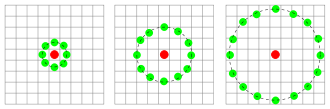
\includegraphics[scale=0.8]{lbp}
	\caption{vecinos en Lbp}
	\label{fig:Vecinos en lbp}
\end{figure}

\newpage

\begin{figure}[h]
	\centering
	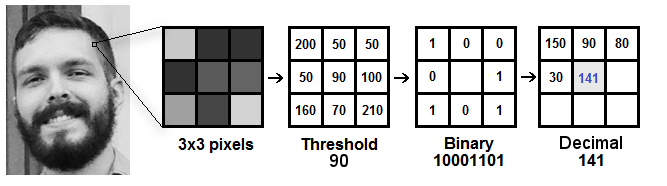
\includegraphics[scale=0.4]{lbpe}
	\caption{Ejemplo de  Lbp}
	\label{fig:Ejemplo}
\end{figure}
\subsubsection{HOG}
El histograma de gradientes orientados (HOG) es un descriptor de características que se utiliza en  visión por computador y en el procesamiento de imágenes para la detección de objetos. tiene dos pasos muy marcados, divide la imagen en un numero definido de celdas y para cada celda obtiene un histograma de la orientación de cada celda en el segundo paso  se calcula los histogramas para todas las celdas luego se combinan para tener la representación global de la imagen en forma de vector de características. 

\begin{figure}[h]
	\centering
	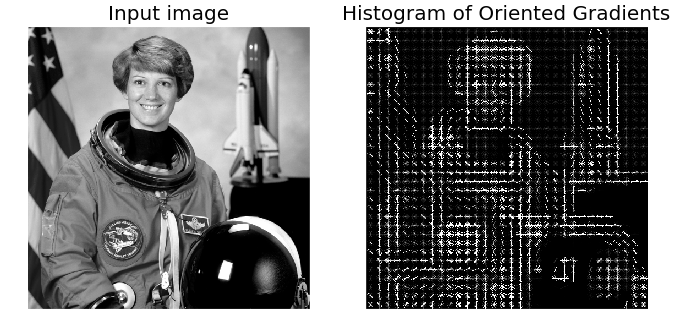
\includegraphics[scale=0.4]{hog.png}
	\caption{Hog}
	\label{fig:Hog}
\end{figure}



\subsection{Descriptores Basados en Movimiento}
\subsubsection{Flujo Óptico}
El flujo óptico puede ser definido como el movimiento aparente de los patrones de intensidad en una imagen. La palabra aparente indica que el movimiento espacial de los objetos (campo de movimiento) puede coincidir o no con el flujo estimado. No obstante, en situaciones en las cuales el movimiento de los objetos implica un movimiento de sus patrones de intensidad en el plano de la imagen, el flujo óptico puede relacionarse directamente con el movimiento de los objetos en la escena

Los algoritmos de flujo óptico tratan de estimar el desplazamiento de un pixel a través de dos consecutivos fotogramas calculando el ángulo de la dirección de su desplazamiento. El resultado que se obtiene es la cantidad de desplazamiento de un pixel en el eje coordenado X y Y.
Dentro de las técnicas de flujo óptico ampliamente utilizadas tenemos:

\begin{itemize}
	\item Lucas - Kanade 
	\item Horn - Shunck
	\item Gunnar Farnebäck
\end{itemize}

\begin{figure}[h]
 \centering
  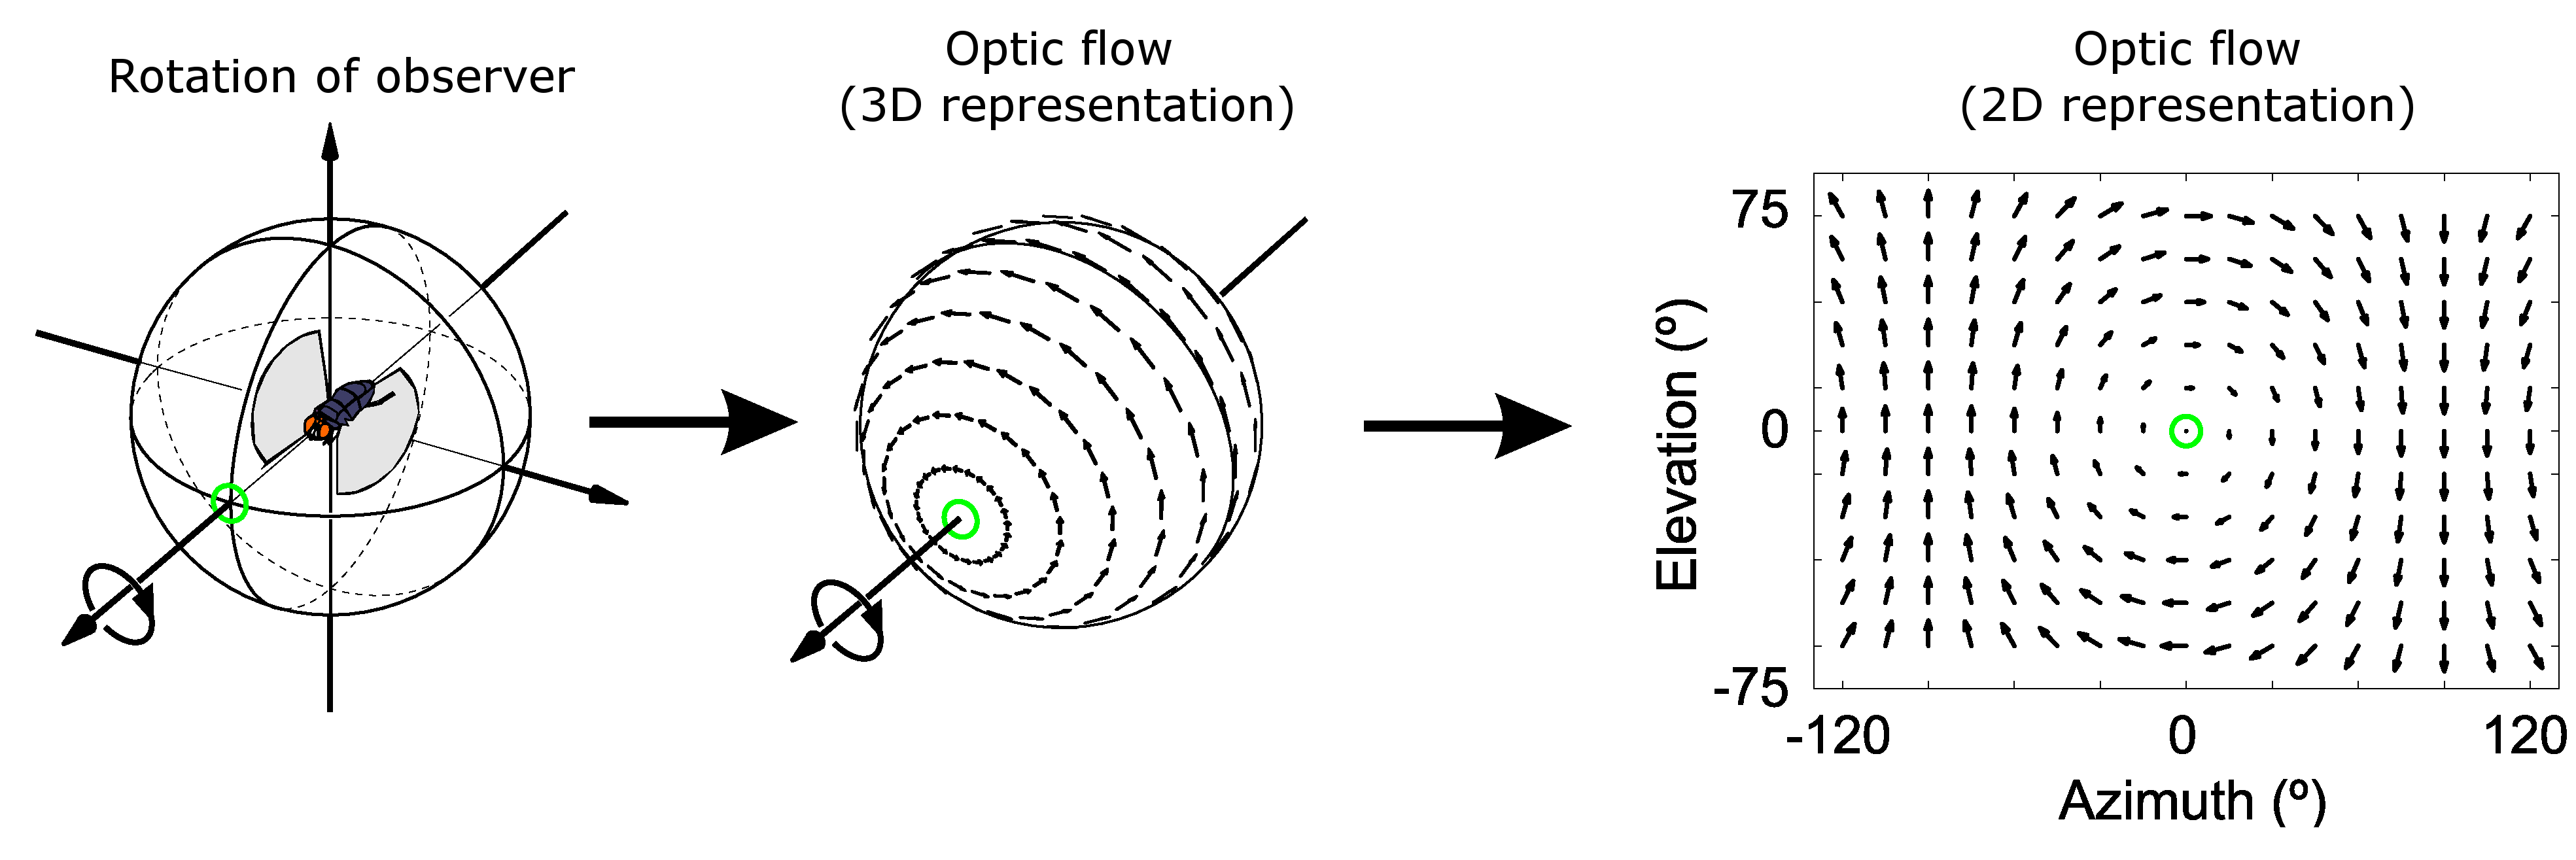
\includegraphics[scale=0.5]{opticFlow}
  \caption{Flujo optico }
  \label{fig:Flujo Optico}
\end{figure}



\section{Clasificadores}


\subsection{Cascadas de Haar}
Propuesto por Viola-Jones, las cascadas de Haar pueden ser  definidas básicamente como un conjunto de regiones rectangulares de sumas a los cuales se les resta otras regiones, las cuales pueden estar presentes en cualquier posición y escala dentro de una imagen. Estas restas son analizadas por clasificadores en cascada, los cuales son un conjunto de clasificadores débiles que trabajando en conjunto para forman un clasificador fuerte, el cual decide qué características son relevantes y cuales tienen que ser rechazadas.

\subsection{Red Neuronal Convolucional}
La arquitectura de una Red Neuronal Convolucional está compuesta por diferentes capas que transforma la entrada en un conjunto de salida.
\begin{figure}[h]
 \centering
  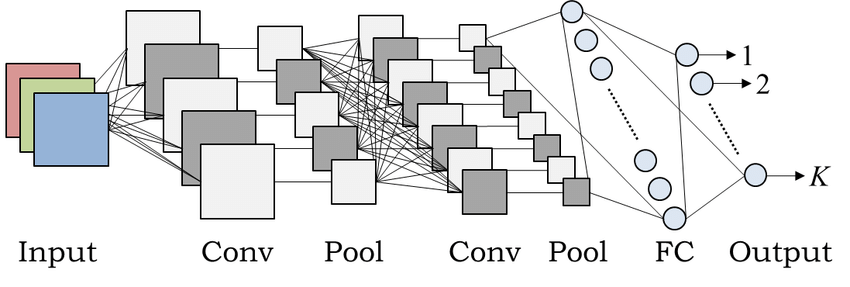
\includegraphics[scale=0.2]{cnn}
  \caption{Arquitectura de una red neuronal convolucional}
  \label{fig:Arquitectura Cnn}
\end{figure}

Capa de convolución es el núcleo principal de la construcción de una Red Neuronal Convolucional. La capa de convolución consiste en un conjunto de neuronas que conecta regiones pequeñas de la entrada con una capa anterior. Estas regiones son llamadas filtros los cuales pueden variar de tamaño.

\begin{figure}[h]
 \centering
  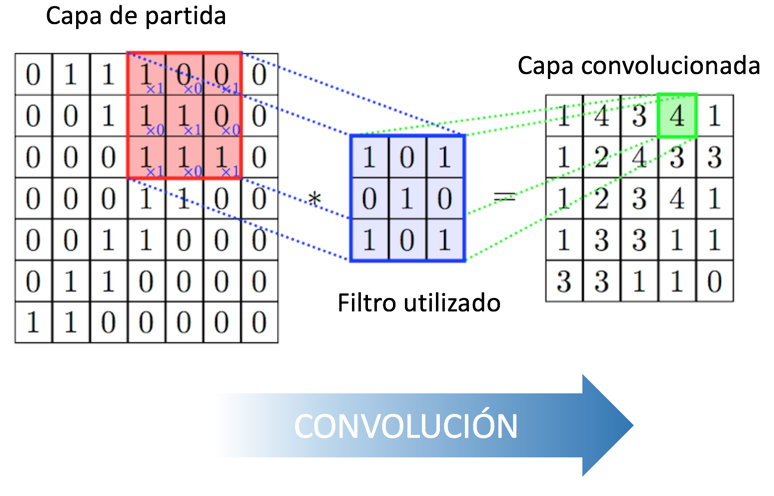
\includegraphics[scale=0.4]{convolucion}
  \caption{Convolucion}
  \label{fig:Convolucion}
\end{figure}



La función de Pooling reduce progresivamente el tamaño espacial de la representación con el objetivo de reducir la cantidad de parámetros y cálculos en la Red. Existen varias funciones

\begin{figure}[h]
 \centering
  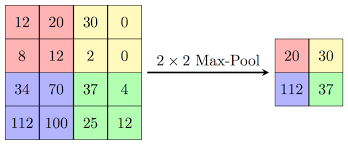
\includegraphics[scale=0.4]{pooling}
  \caption{poolingl}
  \label{fig:pooling}
\end{figure}

\subsection{Support Vector Machine (SVM)}
Está basado en la teoría de aprendizaje propuesto por SVMs son clasificadores lineales, y determinan un límite de decisión mediante un hiperplano. Como puede existir un límite infinito de hiperplanos, uno se puede preguntar cuál de estos hiperplanos es el óptimo en términos de generalizar el clasificador. Por este motivo los SVMs son construidos de tal manera que maximicen la distancia para el conjunto de datos de entrenamiento más cercano de ambas clases.


\begin{figure}[h]
	\centering
	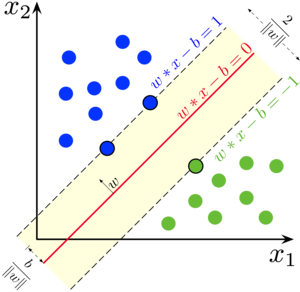
\includegraphics[scale=2]{svm}
	\caption{Support Vector Machine}
	\label{fig:svm}
\end{figure}
\section{Evaluación }
\subsection{Evaluación del clasificador}
\subsubsection{Matriz de confusión}
Matriz de confusión es una herramienta que permite la visualización del desempeño de un algoritmo que se emplea en aprendizaje supervisado. Cada columna de la matriz representa el número de predicciones de cada clase, mientras que cada fila representa a las instancias en la clase real

\begin{figure}[h]
	\centering
	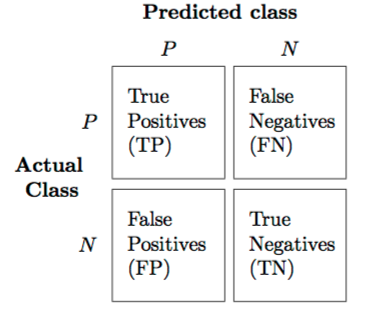
\includegraphics[scale=0.4]{confusion}
	\caption{Matriz de confusionl}
	\label{fig:Matriz de confusion}
\end{figure}

\subsection{Evaluación del detector}
\subsubsection{F-score}
La evaluación del rendimiento del detector será mediante F-score, para eso se tiene que calcular previamente, los falsos positivos, reales positivos, falsos negativos, reales negativos.

\begin{figure}[h]
	\centering
	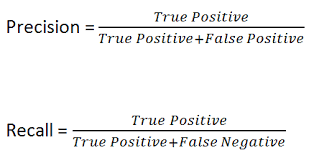
\includegraphics[scale=0.6]{Metodologia}
	\caption{Precision y recall}
	\label{fig:Precision y recall}
\end{figure}

\begin{figure}[h]
	\centering
	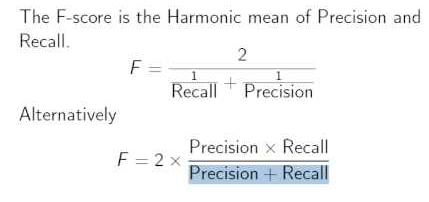
\includegraphics[scale=0.7]{Metodologia2}
	\caption{F-Score}
	\label{fig:F-Score }
\end{figure}



\chapter{Revisión Bibliográfica}



\section{Antecedentes del proyecto }

Durante décadas no se ha avanzado en la detección de avalanchas y sobre todo con técnicas en videos \cite{Christiansen2001},y  uno de los primeros trabajos en los que en los que se usa fotografiá para estudiar el comportamiento de la nieve\cite{Christiansen2001}; existen otros trabajos para monitorerar  deslizamientos de avalanchas con fotografiás estos trabajos tratan de monitorizar el desplazamiento mediante el conteo de pixeles negros en fotografiás continuas generalmente tomadas en un intervalo de 15 minutos \cite{Thesis2014,Herwijnen2012,Herwijnen2013}; también \cite{Herwijnen2012} recomienda, Primero: que el angulo de visión de la cámara y la pendiente deben de estar lo mas cerca posible a  90 grados; Segundo:La cámara deberá de tener buen acercamiento en el área de interés para para obtener mejores datos; Tercero:el intervalo entre imágenes deberían de tener como máximo ya que las avalanchas surgen rápidamente después de las grietas; por lo tanto  se entiende que un monitoreo en tiempo real seria lo ideal no solamente para monitorizar grietas; si no también avalanchas en ese sentido el uso de videos para estudiar eventos anómalos se ha masificado, existen investigaciones que hacen uso de video para el estudio de avalanchas \cite{Akitaya1980,Nishimura1993}; sin embargo solo llegan a registrar estos eventos mas no a detectarlos, considerando los avances tecnológicos, particularmente en inteligencia artificial, se tienen trabajos en pronostico y detección,\cite{Singh2008} hace  uso de redes neuronales artificiales(ANN)y como parámetros de entrada, temperatura del aire, temperatura de la superficie de la nieve, velocidad del viento, etc. los investigadores indican de que ningún modelo puede imitar completamente el método de análisis de un experto, pero con los avances en inteligencia artificial lo modelos están demostrando que son confiables , en  detección de eventos en video por ejemplo \cite{Arceda2015}. presenta un método  para la detección en tiempo real de acciones violentas en secuencias de video con Violent Flow (ViF) y horn-schunk, donde vif es un descriptor y horn-schunk  es un algoritmo de flujo óptico, esta investigación concluye que el método vif horn-shunk tiene buen desempeño reduciendo el tiempo de procesamiento, en otros casos se tiene investigaciones aplicadas a la detección de desastres como es el caso de \cite{Muhammad2019}, que en su investigación comentan las bondades de las redes neuronales convolucionales (CNN) en su desempeño  y lo importante que sería su aplicación y reducir el impacto ecológico y social, al mismo tiempo comentan lo costoso computacionalmente que es utilizarlos es por eso que ellos hace uso de una red SqueezeNet (modelo de red neuronal), respecto  detección de avalanchas en video no se encontraron  investigaciones.


\chapter{Propuesta}



\section{Base de datos}

Se tiene una registro en video del estado de la laguna Palcacocha de Marzo a Julio de 2019,  que se utilizaran para probar el modelo propuesto.

\section{Experimentos}

Luego de implementado los diferentes sistemas de adquisición de datos, se extraerán secuencias de video que superen el umbral de movimiento; previamente se realizara el preprocesamiento de video donde se quitara el ruido producido por lluvias, neblina y el movimiento de la cámara generada por el viento.

Luego se procederá a la extracción de características de los puntos de interés, las lenguas glaciares y las secciones del posible recorrido de la avalancha, se propone experimentar con descriptores  basados en apariencia LBP, HOG (Local Binary patterns
, Histogram Oriented Gradient) y descriptores basados en movimiento HOF, HOOF, HOFG ( Histogram Oriented Flow, Histogram of Oriented Optical Flow, Histogram of optical flow Gradients),  y técnicas complementarias de flujo óptico como el algoritmo Gunnar Farnebäck, Horn - Shunck, Lucas - Kanade  y el descriptor de Flujo Violento; operadores  morfológicos (para remover ruido y separar elementos); se probará también diferentes clasificadores, entre ellos Support Vector Machine, cascadas de haar,Redes neuronales convolucionales. 

Se usará matrices de confusión para la evaluación, comparación del desempeño de los clasificadores, y para la evaluación del detector se utilizara F-score, seleccionando el mejor subconjunto. Las salidas de los modelos de detección de movimiento, se determinará la sensibilidad y precisión. Para finalmente determinar los modelos apropiados al caso estudiado.



\begin{figure}[h]
	\centering
	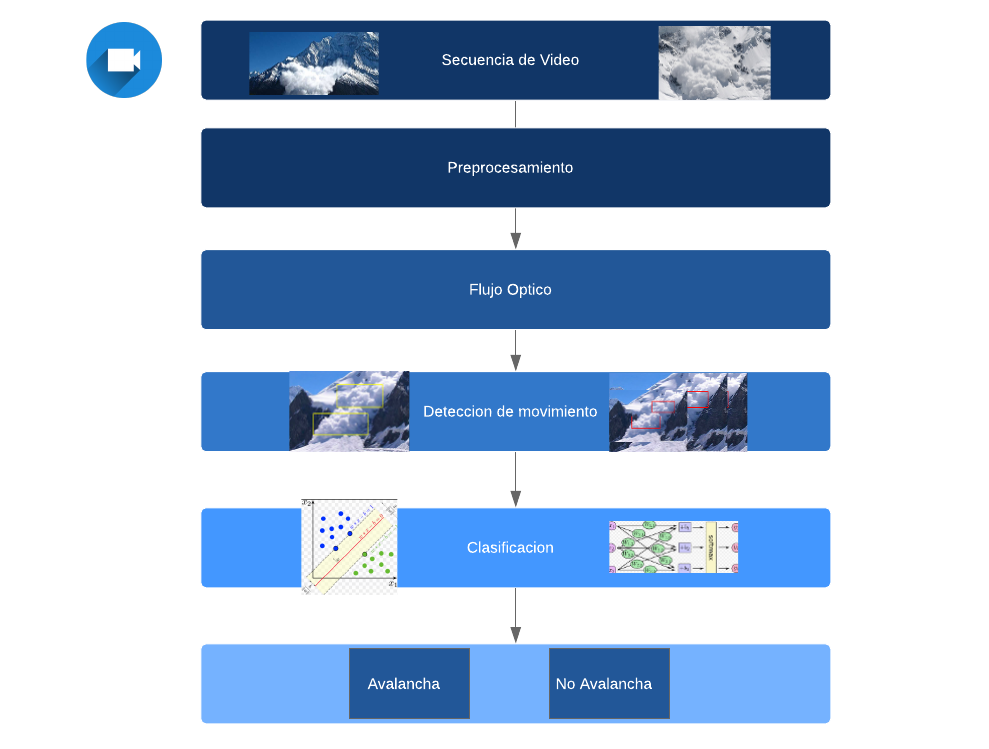
\includegraphics[scale=1.1]{propuesta}
	\caption{Propuesta}
	\label{fig:Propuesta }
\end{figure}




\chapter{Cronograma de Actividades}

\begin{figure}[h]
	\centering
	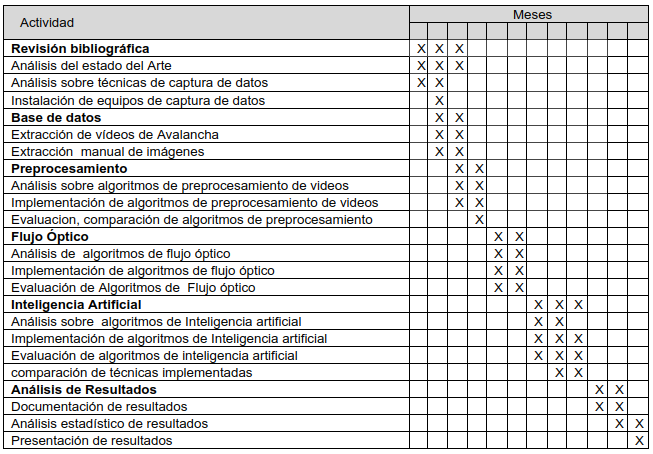
\includegraphics[scale=0.7]{cronograma}
	\caption{Cronograma de actividades}
	\label{fig:Cronograma }
\end{figure}


%\chapter{Referencias}
\bibliographystyle{apacite}
%\bibliographystyle{alpha}
\bibliography{Ref}


\vspace{1cm}

\end{document}
